\documentclass[11pt]{article}

\usepackage[a4paper,margin=1in]{geometry}
\usepackage{amsmath}
\usepackage{amssymb}
\usepackage{caption}
\usepackage{float}
\usepackage{tikz}
\usetikzlibrary{arrows,positioning,calc,backgrounds,fit}

\captionsetup{font=small,labelfont=bf}

%================= colour palette =================
\definecolor{cAmberF}{HTML}{FCEFCF}
\definecolor{cAmberD}{HTML}{B5821E}
\definecolor{cAmberT}{HTML}{6B4E12}
\definecolor{cBlueF}{HTML}{E6F0FB}
\definecolor{cBlueD}{HTML}{5B9BD5}
\definecolor{cBlueT}{HTML}{1C4E80}
\definecolor{cRedF}{HTML}{FBE0DF}
\definecolor{cRedD}{HTML}{C0504D}
\definecolor{cRedT}{HTML}{7A2E2C}
\definecolor{cTealF}{HTML}{DBF1EA}
\definecolor{cTealD}{HTML}{1D9E75}
\definecolor{cTealT}{HTML}{0F6E56}
\definecolor{cGrayF}{HTML}{ECEBE8}
\definecolor{cGrayD}{HTML}{9B9A95}
\definecolor{cGrayT}{HTML}{4A4A46}
\definecolor{cGreenF}{HTML}{E2F0D9}
\definecolor{cGreenD}{HTML}{70AD47}
\definecolor{cGreenT}{HTML}{27500A}
\definecolor{cCoralF}{HTML}{FBE6DC}
\definecolor{cCoralD}{HTML}{D85A30}
\definecolor{cCoralT}{HTML}{993C1D}
\definecolor{cPurpF}{HTML}{EAE8FA}
\definecolor{cPurpD}{HTML}{7F77DD}
\definecolor{cPurpT}{HTML}{3C3489}
\definecolor{leak}{HTML}{C0392B}

%================= tikz styles =================
\tikzset{
  blk/.style   = {rounded corners=2pt, draw, line width=0.6pt, inner sep=4pt,
                  align=center, font=\footnotesize, minimum height=7mm},
  amber/.style = {blk, fill=cAmberF, draw=cAmberD, text=cAmberT},
  gray/.style  = {blk, fill=cGrayF,  draw=cGrayD,  text=cGrayT},
  heater/.style= {blk, fill=cRedF,   draw=cRedD,   text=cRedT,
                  font=\scriptsize, minimum height=5mm, inner sep=2.5pt},
  green/.style = {blk, fill=cGreenF, draw=cGreenD, text=cGreenT,
                  font=\scriptsize, minimum height=5mm, inner sep=2.5pt},
  water/.style = {rounded corners=4pt, draw=cBlueD, line width=0.7pt, dashed,
                  fill=cBlueF, fill opacity=0.55, text opacity=1},
  leakarr/.style = {leak, line width=1pt, -stealth},
  faint/.style   = {cGrayD, line width=0.7pt, densely dashed},
  weak/.style    = {leak, line width=0.8pt, densely dashed, -stealth},
  ground/.pic = {
    \draw[cGrayD, line width=0.6pt] (0,0) -- (0,-0.16);
    \draw[cGrayD, line width=0.6pt] (-0.18,-0.16) -- (0.18,-0.16);
    \draw[cGrayD, line width=0.6pt] (-0.12,-0.25) -- (0.12,-0.25);
    \draw[cGrayD, line width=0.6pt] (-0.06,-0.34) -- (0.06,-0.34);
  },
  vcap/.pic = {
    \draw[cGrayT, line width=1pt] (-0.16,0.045) -- (0.16,0.045);
    \draw[cGrayT, line width=1pt] (-0.16,-0.045) -- (0.16,-0.045);
  },
}

%================= title =================
\title{\textbf{Why a Thermocouple Reads Stably in Air but ``Jumps'' in
Water:\\ A Loop--Cutting View of Common--Mode and Ingress Failure Modes}}
\author{A Technical Note}
\date{\today}

\begin{document}
\maketitle

\begin{abstract}
\noindent A thermocouple that reads steadily in air yet erratically once
immersed is one of the most common bench complaints, and it is almost always
first blamed on a waterproofing defect. We argue that the dominant cause is
electrical rather than mechanical: conductive water closes a leakage--current
loop that develops a \emph{common--mode} voltage at the amplifier input,
driving it out of its linear range. We present a unifying ``loop--cutting''
picture in which every standard remedy---full floating and galvanic
isolation---is merely a different place to break the \emph{same} loop, and we
contrast this electrical family with the genuinely distinct case of water
ingress forming a false junction. Five diagrams illustrate the mechanisms, and
a single bench test is given that separates the two families.
\end{abstract}

\section{The phenomenon}
The thermoelectric (Seebeck) signal of a thermocouple is a differential
voltage of only $\sim\!40~\mu\mathrm{V}/^{\circ}\mathrm{C}$ for a type--K
junction. Because it is so small, the measurement is acutely sensitive to any
voltage that appears \emph{common} to both leads. In still air the leads sit
at a benign potential and the reading is stable. The instant the probe enters
tap water---which is electrically conductive---a new current path appears, and
the reading begins to wander. The reflex diagnosis, ``the probe is not
waterproof,'' is usually wrong.

\section{The leakage loop and the common--mode voltage}
Figure~\ref{fig:loop} shows the mechanism. A mains--powered appliance sharing
the bath (a heater, pump or circulator) leaks a small current into the water.
The water carries that current to the thermocouple, up the leads, into the
amplifier, and back to earth through the instrument's ground, closing a loop.
The leakage current $i_{\ell}$ flowing through the finite impedance to ground
raises both leads together: a common--mode voltage
\[
  V_{cm} \;=\; i_{\ell}\,Z_{\mathrm{gnd}} .
\]
A differential front end rejects common--mode only while its inputs stay
inside their specified range. Once $V_{cm}$ pushes the inputs past the supply
rails (or beyond the part's stated common--mode window), the input protection
conducts, common--mode rejection collapses, and the output is garbage.
Because the leakage is mains--coupled, $V_{cm}$ swings at $50/60~\mathrm{Hz}$;
the sampler catches it at different phases, and aliasing between the
conversion rate and the line frequency produces the characteristic
intermittent ``jumping'' rather than a steady offset.

\begin{figure}[H]
\centering
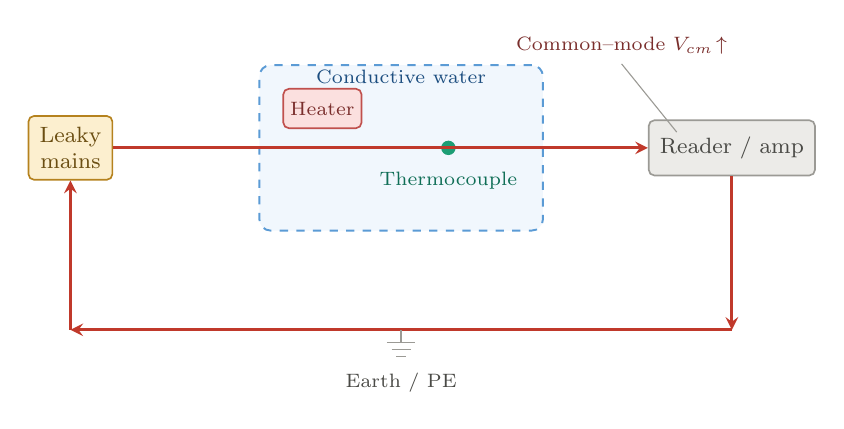
\begin{tikzpicture}[font=\footnotesize]
  \node[amber] (mains) at (0,0) {Leaky\\mains};
  \node[water, minimum width=3.6cm, minimum height=2.1cm] (tank) at (4.2,0) {};
  \node[cBlueT, font=\scriptsize, anchor=north, inner sep=2pt] at (tank.north) {Conductive water};
  \node[heater] (heat) at (3.2,0.5) {Heater};
  \fill[cTealD] (4.8,0) circle (2.6pt);
  \node[cTealT, font=\scriptsize, anchor=north] at (4.8,-0.18) {Thermocouple};
  \node[gray] (amp) at (8.4,0) {Reader / amp};
  % leakage loop
  \draw[leakarr] (mains.east) -- (amp.west);
  \draw[leakarr] (amp.south) -- ++(0,-1.95) coordinate (ampgnd);
  \draw[leakarr] (ampgnd) -- (mains.south |- ampgnd);
  \draw[leakarr] (mains.south |- ampgnd) -- (mains.south);
  \path (tank.south |- ampgnd) pic{ground};
  \node[cGrayT, font=\scriptsize, anchor=north] at ($(tank.south |- ampgnd)+(0,-0.42)$) {Earth / PE};
  \node[cRedT, font=\scriptsize] (vcm) at (7.0,1.3) {Common--mode $V_{cm}\!\uparrow$};
  \draw[cGrayD, line width=0.4pt] (vcm.south) -- (7.7,0.2);
\end{tikzpicture}
\caption{The leakage current (red) closes a loop and stacks a common--mode
voltage $V_{cm}$ across the amplifier input. Every remedy below is just a
different place to cut this ring.}
\label{fig:loop}
\end{figure}

\section{Remedy A: full floating}
The most direct cut is to remove the amplifier's connection to earth entirely:
run the whole reader on a battery (Fig.~\ref{fig:float}). With nothing tying
the instrument to earth, its reference is dragged along by the thermocouple so
that the front end \emph{rides} the water's potential; the common--mode
between the leads and the instrument's own ground stays near zero,
$V_{cm}\approx 0$. The weakness is fragility: connect a single earthed
cable---a USB lead to an earthed PC, for example---and the cut is reconnected,
so the cure holds only while the instrument is a true island.

\begin{figure}[H]
\centering
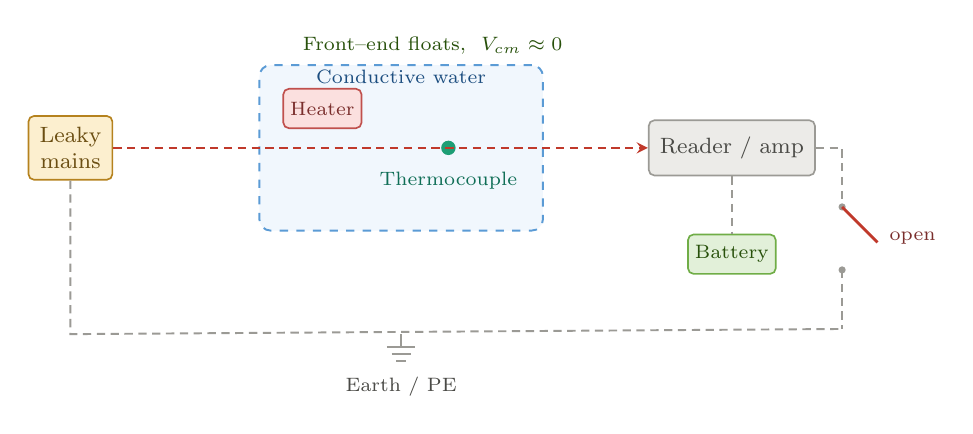
\begin{tikzpicture}[font=\footnotesize]
  \node[amber] (mains) at (0,0) {Leaky\\mains};
  \node[water, minimum width=3.6cm, minimum height=2.1cm] (tank) at (4.2,0) {};
  \node[cBlueT, font=\scriptsize, anchor=north, inner sep=2pt] at (tank.north) {Conductive water};
  \node[heater] (heat) at (3.2,0.5) {Heater};
  \fill[cTealD] (4.8,0) circle (2.6pt);
  \node[cTealT, font=\scriptsize, anchor=north] at (4.8,-0.18) {Thermocouple};
  \node[gray] (amp) at (8.4,0) {Reader / amp};
  \node[green] (bat) at (8.4,-1.35) {Battery};
  \draw[faint] (amp.south) -- (bat.north);
  \draw[weak] (mains.east) -- (amp.west);
  % broken earth path (open switch) on the right
  \draw[faint] (amp.east) -- (9.8,0) -- (9.8,-0.75);
  \fill[cGrayD] (9.8,-0.75) circle (1.3pt);
  \fill[cGrayD] (9.8,-1.55) circle (1.3pt);
  \draw[leak, line width=1pt] (9.8,-0.75) -- (10.25,-1.2);
  \node[cRedT, font=\scriptsize, anchor=west] at (10.28,-1.15) {open};
  \draw[faint] (9.8,-1.55) -- (9.8,-2.3);
  \draw[faint] (mains.south) -- ++(0,-1.95) coordinate (mg) -- (9.8,-2.3);
  \path (tank.south |- mg) pic{ground};
  \node[cGrayT, font=\scriptsize, anchor=north] at ($(tank.south |- mg)+(0,-0.42)$) {Earth / PE};
  \node[cGreenT, font=\scriptsize] at (4.6,1.3) {Front--end floats,\ \ $V_{cm}\approx 0$};
\end{tikzpicture}
\caption{Full floating cuts the amplifier--to--earth segment. The loop cannot
close, so $V_{cm}\approx 0$---but one earthed cable re-closes it.}
\label{fig:float}
\end{figure}

\subsection{The ``fake floating'' trap: Y--capacitors}
A switching DC adapter looks isolated but is not cut cleanly
(Fig.~\ref{fig:ycap}). For EMI compliance it carries Y--capacitors to
protective earth. These block DC but present a low impedance to
mains--frequency AC, so the loop re-closes \emph{weakly} through them. The
common--mode is reduced but not zeroed---the familiar ``much better, yet still
jumps now and then.''

\begin{figure}[H]
\centering
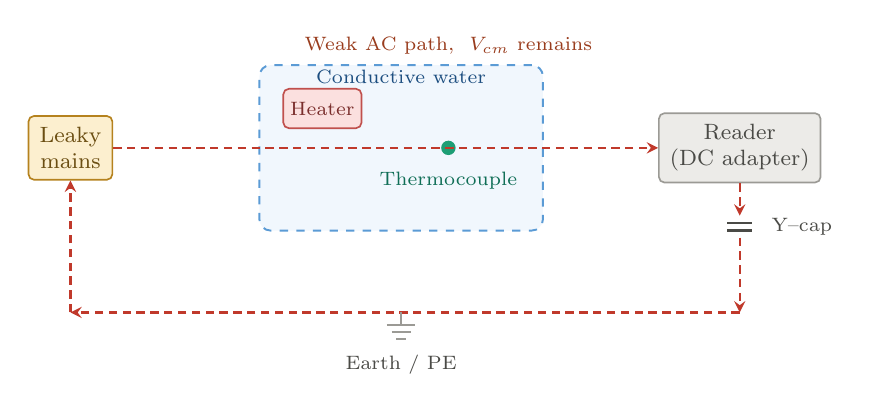
\begin{tikzpicture}[font=\footnotesize]
  \node[amber] (mains) at (0,0) {Leaky\\mains};
  \node[water, minimum width=3.6cm, minimum height=2.1cm] (tank) at (4.2,0) {};
  \node[cBlueT, font=\scriptsize, anchor=north, inner sep=2pt] at (tank.north) {Conductive water};
  \node[heater] (heat) at (3.2,0.5) {Heater};
  \fill[cTealD] (4.8,0) circle (2.6pt);
  \node[cTealT, font=\scriptsize, anchor=north] at (4.8,-0.18) {Thermocouple};
  \node[gray, align=center] (amp) at (8.5,0) {Reader\\(DC adapter)};
  \draw[weak] (mains.east) -- (amp.west);
  \draw[weak] (amp.south) -- (8.5,-0.86);
  \path (8.5,-1.0) pic{vcap};
  \node[cGrayT, font=\scriptsize, anchor=west] at (8.78,-1.0) {Y--cap};
  \draw[weak] (8.5,-1.14) -- ++(0,-0.95) coordinate (mg);
  \draw[weak] (mg) -- (mains.south |- mg);
  \draw[weak] (mains.south |- mg) -- (mains.south);
  \path (tank.south |- mg) pic{ground};
  \node[cGrayT, font=\scriptsize, anchor=north] at ($(tank.south |- mg)+(0,-0.42)$) {Earth / PE};
  \node[cCoralT, font=\scriptsize] at (4.8,1.3) {Weak AC path,\ \ $V_{cm}$ remains};
\end{tikzpicture}
\caption{A Y--capacitor gives mains--frequency AC a weak path to earth, so the
loop is only partly cut and residual $V_{cm}$ survives.}
\label{fig:ycap}
\end{figure}

\section{Remedy B: galvanic isolation}
The robust cut is made \emph{inside} the amplifier (Fig.~\ref{fig:iso}). An
isolation barrier splits the part in two. The front end connects to the
thermocouple and is free to float with the water; the back end stays earthed
and may connect to a PC or any other earthed equipment. The conducted loop
strikes the barrier and cannot cross. This is why isolation beats full
floating: the back end can be tied to earth and to other gear without
re-closing the loop.

\begin{figure}[H]
\centering
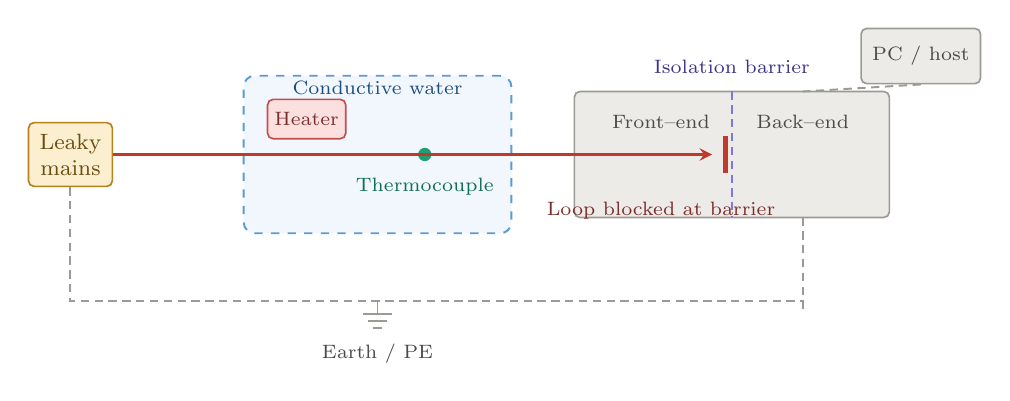
\begin{tikzpicture}[font=\footnotesize]
  \node[amber] (mains) at (0,0) {Leaky\\mains};
  \node[water, minimum width=3.4cm, minimum height=2.0cm] (tank) at (3.9,0) {};
  \node[cBlueT, font=\scriptsize, anchor=north, inner sep=2pt] at (tank.north) {Conductive water};
  \node[heater] (heat) at (3.0,0.45) {Heater};
  \fill[cTealD] (4.5,0) circle (2.4pt);
  \node[cTealT, font=\scriptsize, anchor=north] at (4.5,-0.18) {Thermocouple};
  \node[gray, minimum width=4cm, minimum height=1.6cm] (amp) at (8.4,0) {};
  \node[cGrayT, font=\scriptsize] at (7.5,0.42) {Front--end};
  \node[cGrayT, font=\scriptsize] at (9.3,0.42) {Back--end};
  \draw[cPurpD, densely dashed, line width=0.8pt] (8.4,0.8) -- (8.4,-0.8);
  \node[cPurpT, font=\scriptsize] at (8.4,1.12) {Isolation barrier};
  % red current into front-end, blocked at barrier
  \draw[leakarr] (mains.east) -- (8.15,0);
  \draw[leak, line width=1.8pt] (8.32,0.24) -- (8.32,-0.24);
  \node[cRedT, font=\scriptsize, anchor=north] at (7.5,-0.48) {Loop blocked at barrier};
  % back-end earthed + PC
  \draw[faint] (9.3,-0.8) -- ++(0,-1.2) coordinate (bg);
  \draw[faint] (mains.south) -- ++(0,-1.45) coordinate (mg) -- (mg -| bg) -- (bg);
  \path (tank.south |- mg) pic{ground};
  \node[cGrayT, font=\scriptsize, anchor=north] at ($(tank.south |- mg)+(0,-0.42)$) {Earth / PE};
  \node[gray, font=\scriptsize] (pc) at (10.8,1.25) {PC / host};
  \draw[faint] (pc.south) -- (9.3,0.8);
\end{tikzpicture}
\caption{Galvanic isolation cuts the loop at a barrier inside the chip. The
front end floats with the water; the earthed back end may connect freely.}
\label{fig:iso}
\end{figure}

\section{A distinct failure mode: water ingress}
The four cases above are one disease---a ground loop---cut in four places. The
original suspicion, ``not waterproof,'' is a \emph{different} disease with no
relation to grounding (Fig.~\ref{fig:ingress}). A thermocouple reads wherever
its junction is, normally at the sheath tip. If water penetrates a crack and
bridges the two dissimilar wires partway along, that bridge becomes a new,
wandering junction. The reading then reflects a moving, ill--defined point and
jumps. This is ``not waterproof'' in the literal sense. Two further causes
behave similarly by other mechanisms: unshielded leads picking up ambient EMI,
and a loose or corroded connection.

\begin{figure}[H]
\centering
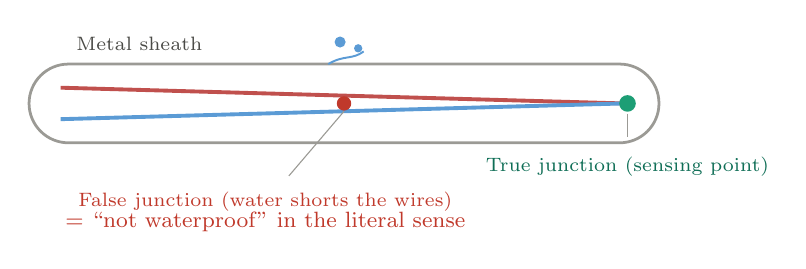
\begin{tikzpicture}[font=\footnotesize]
  % sheath (capsule)
  \draw[cGrayD, line width=1pt, rounded corners=0.5cm] (0,-0.5) rectangle (8,0.5);
  \node[cGrayT, font=\scriptsize, anchor=south] at (1.4,0.55) {Metal sheath};
  % wires
  \draw[cRedD,  line width=1.4pt] (0.4,0.2)  -- (7.55,0);
  \draw[cBlueD, line width=1.4pt] (0.4,-0.2) -- (7.55,0);
  % true junction
  \fill[cTealD] (7.6,0) circle (3pt);
  \node[cTealT, font=\scriptsize, anchor=north] at (7.6,-0.55) {True junction (sensing point)};
  \draw[cGrayD, line width=0.4pt] (7.6,-0.13) -- (7.6,-0.42);
  % water droplets at crack (x = 4)
  \fill[cBlueD] (3.95,0.78) circle (2pt);
  \fill[cBlueD] (4.18,0.7)  circle (1.5pt);
  \draw[cBlueD, line width=0.7pt] (3.8,0.5) .. controls (4.0,0.62) and (4.1,0.55) .. (4.25,0.66);
  % false junction (water shorts the two wires)
  \draw[leak, line width=2.4pt] (4,0.087) -- (4,-0.087);
  \fill[leak] (4,0) circle (2.6pt);
  \node[leak, font=\scriptsize, anchor=north] at (3.0,-1.0) {False junction (water shorts the wires)};
  \draw[cGrayD, line width=0.4pt] (4,-0.1) -- (3.3,-0.92);
  \node[leak, font=\footnotesize] at (3.0,-1.5) {$=$ ``not waterproof'' in the literal sense};
\end{tikzpicture}
\caption{Ingress mode: water bridges the wires before the tip, creating a
wandering false junction. Grounding fixes do nothing here.}
\label{fig:ingress}
\end{figure}

\section{Diagnosis and summary}
The five figures collapse to two statements.

\emph{The first four are one disease}---ground loop / common--mode. The red
ring is the leakage current and $V_{cm}$ is what it stacks up at the input.
Full floating, the Y--capacitor case, and galvanic isolation differ only in
\emph{where} the ring is cut and \emph{how cleanly}: full floating cuts at the
amplifier--to--earth segment (clean but fragile); the Y--capacitor leaves an
AC path (incompletely cut); isolation cuts at the in--chip barrier (robust,
and it leaves the back end free to be earthed).

\emph{The fifth is a different disease}---genuine water ingress, which forms a
false junction and is untouched by any grounding measure.

A one--line bench test separates them: \textbf{wipe the probe dry and read it.}
If it is stable immediately, the fault is electrical (one of the first four)
and the seal is fine. If it recovers only after a long dry--out, water has
gotten inside (the fifth). Two confirmatory checks: jumping that is
synchronous with an appliance switching points to the loop or to transient
coupling; jumping that changes when the leads are twisted or shortened points
to differential pickup.

\end{document}
